\documentclass[notes,blackandwhite,mathsans,usenames,dvipsnames]{beamer}

\usepackage{amsmath}
\usepackage{amssymb}
\usepackage{graphicx}
\usepackage{fancybox}
\usepackage{booktabs}
\usepackage{multirow,pxfonts}
\usepackage{cmbright}
\usepackage{xcolor}
\usepackage{color}
\usepackage{enumitem}
\usepackage{animate}
\usepackage{changepage}

\usepackage[T1]{fontenc}
\fontencoding{T1}  
\usepackage[utf8]{inputenc}


\usefonttheme{default}
\setbeamercovered{invisible}
\beamertemplatenavigationsymbolsempty

\makeatletter
\setbeamertemplate{footline}
{
  \leavevmode
  \hbox{
  \begin{beamercolorbox}[wd=0.97\paperwidth,ht=2.25ex,dp=2ex,right]{}
{\color{mcxs2} \insertframenumber{} / \inserttotalframenumber}
  \end{beamercolorbox}}%
}



\definecolor{mcxs1}{HTML}{05386B}
\definecolor{mcxs2}{HTML}{379683}
\definecolor{mcxs3}{HTML}{5CDB95}
\definecolor{mcxs4}{HTML}{8EE4AF}
\definecolor{mcxs5}{HTML}{EDF5E1}
\setbeamercolor{frametitle}{fg=mcxs2}
\AtBeginDocument{\color{mcxs1}}

\setbeamercolor{itemize item}{fg=mcxs1}
\setbeamercolor{itemize subitem}{fg=mcxs2}
\setbeamercolor{enumerate item}{fg=mcxs1}
\setbeamercolor{description item}{fg=mcxs1}

\setbeamertemplate{itemize item}[triangle]
\setbeamertemplate{itemize subitem}[circle]




\begin{document}
%\fontfamily{pag}\selectfont
%\setbeamerfont{title}{family=\fontfamily{pag}\selectfont}
%\setbeamerfont{frametitle}{family=\fontfamily{pag}\selectfont}
%\setbeamerfont{framesubtitle}{family=\fontfamily{pag}\selectfont}







{\setbeamercolor{background canvas}{bg=purple}
\begin{frame}

\vspace{1cm}
\begin{tabular}{rl}
&\textbf{\LARGE\color{mcxs2} Macroeconometrics}\\[8ex]
\textbf{\Large Lecture 10}&\textbf{\Large\color{mcxs5}Forecasting with}\\
&\textbf{\Large\color{mcxs5}Large Bayesian VARs}\\[16ex]
&\textbf{Tomasz Wo\'zniak}\\[1ex]
&{\small\color{mcxs5} Department of Economics}\\
&{\small\color{mcxs5}University of Melbourne}
\end{tabular}

\end{frame}
}






\begin{frame}

\bigskip\textbf{\color{purple}Large Bayesian VARs}

\bigskip\textbf{\color{mcxs2}Sampling from the posterior density}

\bigskip\textbf{\color{mcxs2}Sampling from predictive density}

\bigskip\textbf{\color{mcxs2}Feasible computations}

\bigskip\textbf{\color{purple}Forecasting Australian real output and inflation using fat data}


\small
\bigskip References: \scriptsize

\smallskip{\color{mcxs2}Panagiotelis, Athanasopoulos, Hyndman, Jiang, Vahid (2019) Macroeconomic forecasting for Australia using a large number of predictors, International Journal of Forecasting}

\smallskip{\color{mcxs2}Ba\'nbura, Giannone, Reichlin (2010) Large Bayesian Vector Auto Regressions, Journal of Applied Econometrics}

\small
\bigskip Materials: \scriptsize

\smallskip{\color{mcxs2}R files} \texttt{L10 mcxs-N2.R} {\color{mcxs2}and} \texttt{L10 mcxs-N117.R} {\color{mcxs2}for the reproduction of the results}

\smallskip{\color{mcxs2}Data file} \texttt{ausmacrodata-2016.csv}
\end{frame}






{\setbeamercolor{background canvas}{bg=purple}
\begin{frame}

\bigskip\textbf{\color{mcxs1}Objectives.}
\begin{itemize}[label=$\blacktriangleright$]
\item {\color{mcxs1}To introduce challenges of working with fat data}
\item {\color{mcxs1}To present Bayesian solutions to overparemeterised models}
\item {\color{mcxs1}To forecast output and prices using 117 variables}
\end{itemize}

\bigskip\textbf{\color{mcxs5}Learning outcomes.}
\begin{itemize}[label=$\blacktriangleright$]
\item {\color{mcxs5}Understanding some computational challenges of working with large data}
\item {\color{mcxs5}Forecasting with Bayesian VARs}
\item {\color{mcxs5}Verifying the computational time of alternative routines}
\end{itemize}

\end{frame}
}




{\setbeamercolor{background canvas}{bg=purple}
\begin{frame}

\begin{adjustwidth}{-0.5cm}{0cm}
\vspace{8.3cm}\Large
\textbf{{\color{mcxs1}Large} {\color{white}Bayesian VARs}}
\end{adjustwidth}

\end{frame}
}





\begin{frame}{Bayesian VARs}

\textbf{Posterior density.}
\begin{align*} 
p\left( {\color{purple}A}, {\color{purple}\Sigma}|Y,X \right) &= p({\color{purple}A}|Y,X,{\color{purple}\Sigma})p\left( {\color{purple}\Sigma}|Y,X \right)\\[2ex]
p({\color{purple}A}|Y,X,{\color{purple}\Sigma}) &= \mathcal{MN}_{K\times N}\left( \overline{A},{\color{purple}\Sigma},\overline{V} \right)\\
p({\color{purple}\Sigma}|Y,X) &= \mathcal{IW}_N\left( \overline{S}, \overline{\nu} \right)\\[2ex]
\overline{V}&= \left( X'X + \underline{V}^{-1}\right)^{-1} \\
\overline{A}&= \overline{V}\left( X'Y + \underline{V}^{-1}\underline{A} \right)\\
\overline{\nu}&= T+\underline{\nu}\\
\overline{S}&= \underline{S}+Y'Y + \underline{A}'\underline{V}^{-1}\underline{A} - \overline{A}'\overline{V}^{-1}\overline{A}
\end{align*} 

\end{frame}




\begin{frame}{Large Bayesian VARs}

\textbf{Fat data problem.}

{\color{mcxs2}Large Bayesian VARs are defined by the infeasibility of the OLS estimation. The problem arises when the number of variables} $N$ {\color{mcxs2}is large compared to the length of time series} $T${\color{mcxs2}, that is, when} $1+pN>T$

\bigskip {\color{mcxs2}The infeasibility of the OLS estimation comes from the} {\color{purple}reduced rank} {\color{mcxs2}of} $X'X$ {\color{mcxs2}which then cannot be inverted.}

\bigskip
\textbf{Macroeconomic forecasting.}\\
{\color{mcxs2}Consider a system of monthly macro-aggregates for monetary policy in the U.S. The data are available from} 1959{\color{mcxs2}, which gives} $T\approx750$. {\color{mcxs2}Consider VAR(12). In such a case, solving} $K=1+pN<T$ {\color{mcxs2}gives} $N<63$.\\ 
{\color{mcxs2}However, more than a hundred relevant variables, potentially useful for forecasting, is included in panels of data.}
\end{frame}





\begin{frame}{Large Bayesian VARs}

{\color{mcxs2}Large Bayesian VARs are feasible because it is not} $X'X$ {\color{mcxs2}to be inverted, but rather matrix:}
$$ X'X + \underline{V}^{-1} $$
{\color{mcxs2}where} $\underline{V}^{-1}$ {\color{mcxs2}is a positive definite matrix.}

\bigskip 
\textbf{Useful result.}\\
{\color{mcxs2}A sum of a positive definite matrix and a singular matrix gives a~positive definite matrix.}

\bigskip\textbf{Forecasting.}\\
{\color{mcxs2}Many variables may be used for forecasting with Bayesian VARs.}

\end{frame}




\begin{frame}{Large Bayesian VARs: Minnesota prior}

{\color{mcxs2}Let the prior mean assume a random walk process:} 
$$\underline{A}=\begin{bmatrix} \mathbf{0}_{N\times1} & I_N & \mathbf{0}_{N\times(p-1)N}\end{bmatrix}'$$

{\color{mcxs2}Posterior mean of matrix} $A$ {\color{mcxs2}is:}
\begin{align*}
\overline{A} &= {\color{mcxs2}\overline{V}}\left( X^{'}Y + {\color{mcxs2}\underline{V}^{-1}}\underline{A} \right)\\ 
&= {\color{mcxs2}\overline{V}}\left( {\color{mcxs2}X^{'}X}\hat{A} + {\color{mcxs2}\underline{V}^{-1}}\underline{A} \right)\\ 
&= {\color{mcxs2}\overline{V} X^{'}X}\hat{A} + {\color{mcxs2}\overline{V}\underline{V}^{-1}}\underline{A} 
\end{align*}
{\color{mcxs2}a linear combination of the MLE} $\hat{A}$ {\color{mcxs2}and the prior mean} $\underline{A}$

\end{frame}



\begin{frame}{Large Bayesian VARs: Minnesota prior}

\bigskip\textbf{Reduced rank of $X'X$ problem.}\\
{\color{mcxs2}Reduced rank of $X'X$ means that there is not sufficient information in data to inform the estimation of all of the parameters of $A$ matrix. This matrix is not fully identified.

\smallskip The feasibility of Bayesian estimation comes from additional identification information coming from prior distribution.}


\bigskip\textbf{Forecasting using Minnesota prior.}\\
{\color{mcxs2}As long as the information from data is sufficient we predict with an estimated model with parameter estimates} $\hat{A}$.

\smallskip{\color{mcxs2}Whenever the data is not informative about the parameters we predict with a random walk model with parameters} $\underline{A}$
\end{frame}







{\setbeamercolor{background canvas}{bg=purple}
\begin{frame}

\begin{adjustwidth}{-0.5cm}{0cm}
\vspace{8.3cm}\Large
\textbf{{\color{mcxs1}Sampling from} {\color{mcxs5}the posterior density}}
\end{adjustwidth}

\end{frame}
}




\begin{frame}{Sampling from multivariate normal distribution}

{\color{mcxs2}Let an} $N${\color{mcxs2}-vector} $X$ {\color{mcxs2}follow normal distribution. To draw }
$$ X\sim\mathcal{N}_N(\mu,\Sigma) $$

\begin{description}
\item[Sample] {\color{mcxs2}independently} $N$ {\color{mcxs2}draws from a standard normal distribution}
$x_n\sim\mathcal{N}(0,1)$ {\color{mcxs2}and create vector} $\tilde{X} = (x_1, \dots, x_N)$
\bigskip\item[Compute] $S=\text{chol}(\Sigma)$ {\color{mcxs2}a Cholesky decomposition of} $\Sigma$ {\color{mcxs2}such that} $S$ {\color{mcxs2}is lower-triangular and} $\Sigma = SS'$
\bigskip\item[Return] $\mu + S\tilde{X}$ {\color{mcxs2}as a draw from} $\mathcal{N}_N(\mu,\Sigma)$
\end{description}

\bigskip{\color{mcxs2}In R you might use} \texttt{rmvnorm} {\color{mcxs2}function from package} \texttt{mvrnorm}

\end{frame}



\begin{frame}{Sampling from matrix-variate normal distribution}

{\color{mcxs2}Let a} $K\times N$ {\color{mcxs2}matrix} $X$ {\color{mcxs2}follow a matrix-variate normal distribution. To draw} 
$$ X\sim\mathcal{MN}_{K\times N}(M,Q,P) $$

\begin{description}
\item[Sample] {\color{mcxs2}independently} $KN$ {\color{mcxs2}draws from a standard normal distribution}
$x_{k.n}\sim\mathcal{N}(0,1)$ {\color{mcxs2}and create} $K\times N$ {\color{mcxs2}matrix} $\tilde{X}$ {\color{mcxs2}collecting the draws}
\bigskip\item[Compute] $L=\text{chol}(Q)$ {\color{mcxs2}and} $C=\text{chol}(P)$ {\color{mcxs2}such that}  $Q = LL'$ {\color{mcxs2}and} $P = CC'$
\bigskip\item[Return] $M + C\tilde{X}L'$ {\color{mcxs2}as a draw from} $\mathcal{MN}_{K\times N}(M,Q,P)$
\end{description}

\bigskip{\color{mcxs2}For small $K$ and $N$ you might use a simple R code:} \footnotesize
\texttt{matrix(rmvnorm(1, mean=as.vector(M), sigma=Q\%x\%P), ncol=N)}

\end{frame}





\begin{frame}{Sampling from inverse Wishart distribution}

{\color{mcxs2}Let an} $N\times N$ {\color{mcxs2}positive definite matrix} $X$ {\color{mcxs2}follow an inverse Wishart distribution. To draw} 
$$ X\sim\mathcal{IW}_{N}(S,\nu) $$

\begin{description}
\item[Compute] $L=\text{chol}(S)$ {\color{mcxs2}such that}  $S = LL'$

\bigskip\item[Create] $N\times N$ {\color{mcxs2}lower-triangular matrix} $Q$ {\color{mcxs2}by}
	\begin{description}
	\item[setting] {\color{mcxs2}its diagonal elements to} $q_{nn}=\sqrt{c_{nn}}$ {\color{mcxs2}where} $c_{nn}\sim\chi^2_{\nu-n+1}$ {\color{mcxs2}for} $n=1,\dots,N$
	\item[setting] {\color{mcxs2}its elements under the main diagonal to} $q_{mn}\sim\mathcal{N}(0,1)$ {\color{mcxs2}for} $m>n$
	\end{description}

\bigskip\item[Return] $LQ^{-1\prime}Q^{-1}L'$ {\color{mcxs2}as a draw from} $\mathcal{IW}_{N}(S,\nu)$
\end{description}


\end{frame}




\begin{frame}{Sampling from inverse Wishart distribution}


$$ X\sim\mathcal{IW}_{N}(S,\nu) $$

\bigskip{\color{mcxs2}For small $N$ you might use an R function} \texttt{rWishart} {\color{mcxs2}as follows} \footnotesize

\bigskip\texttt{solve(rWishart(1, df=nu, Sigma=solve(S))[,,1])}

\end{frame}




\begin{frame}{Sampling from normal-inverse Wishart distribution}

{\color{mcxs2}To sample} $S$ {\color{mcxs2}random draws from the distribution}
\begin{align*} 
p({\color{purple}A}|Y,X,{\color{purple}\Sigma}) &= \mathcal{MN}_{K\times N}\left( \overline{A},{\color{purple}\Sigma},\overline{V} \right)\\
p({\color{purple}\Sigma}|Y,X) &= \mathcal{IW}_N\left( \overline{S}, \overline{\nu} \right)
\end{align*} 

\begin{description}
\item[Sample] $S$ {\color{mcxs2}independent draws from inverse Wishart distribution:}\\ \small
\texttt{Sigma.inv.posterior = rWishart(S,\\ \hspace{1cm} df=nu.bar,\\ \hspace{1cm} Sigma=solve(S.bar))\\
Sigma.posterior = apply(Sigma.inv.posterior, 3, solve)}

\bigskip\normalsize\item[For each] {\color{mcxs2}draw of} $\Sigma$ {\color{mcxs2}sample a draw of} $A$\\ \small
\texttt{A.posterior = array(NA,c(K,N,S))\\
for (s in 1:S)\{\\
\hspace{1cm}A.posterior[,,s] = rmvnorm(1,\\
\hspace{1.5cm}mean=as.vector(A.bar),\\
\hspace{1.5cm}sigma=Sigma.posterior[,,s]\%x\%V.bar)\\
\hspace{1cm}\} }
\end{description}

\end{frame}



{\setbeamercolor{background canvas}{bg=purple}
\begin{frame}

\begin{adjustwidth}{-0.5cm}{0cm}
\vspace{8.3cm}\Large
\textbf{{\color{mcxs1}Sampling from} {\color{mcxs2}predictive density}}
\end{adjustwidth}

\end{frame}
}




\begin{frame}{Predictive density: Bayesian approach}

\textbf{Joint predictive density.}

\begin{align*} 
p\left(Y_{t+h}\big|Y_t\right) = \int &p\left(Y_{t+h}\big|Y_t, {\color{purple}A},{\color{purple}\Sigma}\right)p\left( {\color{purple}A}, {\color{purple}\Sigma}|Y,X \right) d({\color{purple}A}, {\color{purple}\Sigma}) \\[2ex]
p\left(Y_{t+h}\Big|Y_t,Y,X, {\color{purple}A},{\color{purple}\Sigma}\right) &= \mathcal{N}_{hN}\left(Y_{t+h|t}({\color{purple}A}), \mathbb{V}\text{ar}\left[Y_{t+h|t}\big| {\color{purple}A},{\color{purple}\Sigma}\right]\right)\\
p\left( {\color{purple}A}, {\color{purple}\Sigma}|Y,X \right) &= \mathcal{NIW}_{K\times N}\left( \overline{A},\overline{V}, \overline{S}, \overline{\nu} \right)
\end{align*} 

\end{frame}




\begin{frame}{Predictive density: Bayesian approach}

\textbf{Joint predictive density.}

{\color{mcxs2}Ignore the conditioning on} $Y,X, {\color{purple}A},{\color{purple}\Sigma}$ {\color{mcxs2}in the notation}\small

\begin{align*} 
p\left(Y_{t+h}\big| Y_t\right) &= p\left(\left(y_{t+h}, y_{t+h-1}, \dots, y_{t+2}, y_{t+1}\right) \big| Y_t \right)\\
&= p\left( y_{t+h}\big|y_{t+h-1},\dots,y_{t+1}, Y_t \right) \dots p\left( y_{t+2}\big|y_{t+1}, Y_t \right)p\left( y_{t+1}\big| Y_t \right)\\
\end{align*} 

{\color{mcxs2}where the densities on the right-hand side are }
$$p\left( y_{t+i}\big|y_{t+i-1},\dots,y_{t+1}, Y_t \right) = \mathcal{N}_N\left(\mu_0 + A_1 y_{t+i-1}+\dots+A_py_{t+i-p-1}  ,\Sigma\right)$$

\bigskip{\color{mcxs2}The decomposition above suggests an iterative structure of the algorithm for sampling from the joint predictive density}
\end{frame}



\begin{frame}{Predictive density: Bayesian approach}

\textbf{Sampling from the joint predictive density (Algorithm 2).}

\bigskip 
\begin{description}
\item[Sample] {\color{mcxs2}draws from} $p({\color{purple}A}, {\color{purple}\Sigma}|Y,X)$ {\color{mcxs2}and} 

\bigskip\item[Obtain] $\left\{ A^{(s)}, \Sigma^{(s)}\right\}_{s=1}^{S}$

\bigskip\item[For each] draw of parameters draw from the predictive density
	\begin{description}
	\item[Sample] $y_{t+1}^{(s)}\sim\mathcal{N}_N\left( \mu_0^{(s)} + A_1^{(s)} y_{t}+\dots+A_p^{(s)}y_{t-p} ,\Sigma^{(s)}\right)$
	\item[Sample] $y_{t+2}^{(s)}\sim\mathcal{N}_N\left( \mu_0^{(s)} + A_1^{(s)} y_{t+1}^{(s)}+\dots+A_p^{(s)}y_{t-p+1} ,\Sigma^{(s)}\right)$
	\item[]$\quad\vdots$
	\item[Sample] $y_{t+h}^{(s)}\sim\mathcal{N}_N\left( \mu_0^{(s)} + A_1^{(s)} y_{t+h-1}^{(s)}+\dots+A_p^{(s)}y_{t-p+h}^{(s)} ,\Sigma^{(s)}\right)$
	\end{description}


\bigskip\item[Obtain] $\left\{ y_{t+1}^{(s)},\dots,y_{t+h}^{(s)}\right\}_{s=1}^{S}$

\end{description}

\end{frame}





{\setbeamercolor{background canvas}{bg=purple}
\begin{frame}

\begin{adjustwidth}{-0.5cm}{0cm}
\vspace{8.3cm}\Large
\textbf{{\color{mcxs1}Feasible} {\color{mcxs5}computations}}
\end{adjustwidth}

\end{frame}
}







\begin{frame}{Large Bayesian VARs: feasible estimation}

\textbf{Inverting a matrix.}\\
{\color{mcxs2}Computer algorithms perform} $\mathcal{O}\left(N^3\right)$ {\color{mcxs2}to invert an} $N\times N$ {\color{mcxs2}matrix}

\bigskip\textbf{The Kroneckers.}\\
{\color{mcxs2}To invert the covariance matrix of a matrix-variate normal  posterior distribution apply} 
$$\left(\Sigma\otimes\overline{V}\right)^{-1}= \Sigma^{-1}\otimes\overline{V}^{-1}$$
{\color{mcxs2}which requires} $\mathcal{O}\left(N^3\right) + \mathcal{O}\left(K^3\right)$ {\color{mcxs2}operations which is much less than} $\mathcal{O}\left((NK)^3\right)$ {\color{mcxs2}that would be required if the whole posterior covariance matrix of} $\text{vec}(A)$ {\color{mcxs2}was to be inverted.}

\bigskip\textbf{The Kroneckers.}\\
{\color{mcxs2}Specify their VARs to exploit the Kronecker structure of the covariance matrix.}

\end{frame}



\begin{frame}[fragile]{Large Bayesian VARs: feasible estimation}

\scriptsize
\begin{verbatim}
> library(microbenchmark)
> N       = 10
> p       = 12

> Sigma     = rWishart(1,N+2,diag(N))[,,1]
> XX        = rWishart(1,p*N+3,diag(1+p*N))[,,1]

> microbenchmark(
+   reg   = solve(kronecker(Sigma,XX)),
+   kro = kronecker(solve(Sigma),solve(XX))
+ )
Unit: milliseconds
expr       min         lq       mean    median         uq        max neval
reg 1242.10252 1255.08545 1284.60924 1266.8586 1299.67269 1520.73370   100
kro   12.01087   12.47831   17.86607   13.5652   19.76565   85.75414   100
\end{verbatim}

\normalsize\bigskip
{\color{mcxs2}On average the computations are around 72 times faster}

\end{frame}






\begin{frame}{Large Bayesian VARs: feasible estimation}

\textbf{Inverting a precision matrix.}
$$ \overline{V}^{-1} = X'X + \underline{V}^{-1} $$
{\color{mcxs2}Requires computation of} $\text{det}\big(\overline{V}^{-1}\big)$ {\color{mcxs2}which can be too small for computer's precision of saving numbers to store it in the memory.}

\bigskip\textbf{Apply standarisation.}
\begin{description}
\item[Step 1] {\color{mcxs2}Divide the precision matrix by a constant} $\frac{1}{c_v}\overline{V}^{-1}$ 
\item[Step 2] {\color{mcxs2}Invert} $\big(\frac{1}{c_v}\overline{V}^{-1}\big)^{-1}$
\item[Step 3] {\color{mcxs2}Compute} $\overline{V} = \frac{1}{c_v}\big(\frac{1}{c_v}\overline{V}^{-1}\big)^{-1}$
\end{description}

\bigskip{\color{mcxs2}Choose} $c_v$ {\color{mcxs2}so that the computations are feasible.\\ Try such values as} $c_v=\text{tr}\big(\overline{V}^{-1}\big)$ {\color{mcxs2}or} $c_v=\prod_{k=1}^{K}\big(\overline{V}^{-1}\big)_{k.k}$
\end{frame}






\begin{frame}{Large Bayesian VARs: feasible estimation}

\textbf{Inverting prior covariance matrix.}

{\color{mcxs2} Prior covariance matrix} $\underline{V}$ {\color{mcxs2}is often specified as a diagonal matrix.} 

\bigskip\textbf{Inverting a diagonal matrix.}

{\color{mcxs2}The inverse of a diagonal matrix is equal to a diagonal matrix with its diagonal elements set to the inverses of the diagonal elements of the matrix to be inverted.}

\bigskip\textbf{Inverting a diagonal matrix in R.}

\texttt{V.prior.inv = diag(1/diag(V.prior))}
\end{frame}




\begin{frame}[fragile]{Large Bayesian VARs: feasible estimation}

\scriptsize
\begin{verbatim}
> K       = 1 + p*N
> V.inv   = diag(rgamma(K,1,1))

> microbenchmark(
+   regular   = solve(V.inv),
+   diagonal  = diag(1/diag(V.inv))
+ )
Unit: microseconds
     expr     min       lq     mean   median      uq      max neval
  regular 394.341 532.6595 559.7343 555.2675 586.169 1019.535   100
 diagonal   8.691  38.7660  55.2882  59.1645  68.725  153.467   100
\end{verbatim}

\normalsize\bigskip
{\color{mcxs2}On average the computations are around 10 times faster}

\end{frame}






\begin{frame}{Large Bayesian VARs: feasible estimation}

{\color{mcxs2}A sparse matrix is a matrix with a large fraction of zero elements. Defining a matrix as a sparse allows R to perform less operations to compute the inverse of a matrix.}

\bigskip\textbf{Computing $\overline{A}$ applying operations on triangular matrices.}

{\color{mcxs2}Inverting} $K\times K$ {\color{mcxs2}matrix} $\overline{V}^{-1}$ {\color{mcxs2}to compute} $\overline{A}$ {\color{mcxs2}requires} $\mathcal{O}\left(K^3\right)$ {\color{mcxs2}operations.} 

\bigskip{\color{mcxs2}Inverting a triangular matrix using dedicated programs may cut down the number of operations to} $\mathcal{O}\left(K\right)$

\bigskip$\overline{V}^{-1}$ {\color{mcxs2}is not triangular, however, its Cholesky decomposition is an upper-triangular matrix.}

\end{frame}


\begin{frame}{Large Bayesian VARs: feasible estimation}

\bigskip\textbf{Computing $\overline{A}$ applying operations on triangular matrices.}
\begin{align*} 
\overline{V}^{-1}&=  X'X + \underline{V}^{-1} \\
C &= \text{Chol}\left(\overline{V}^{-1}\right)\text{ such that } \overline{V}^{-1}=C'C\\
\downarrow&\\
\overline{A}&= \overline{V}\left( X'Y + \underline{V}^{-1}\underline{A} \right)\\
&= C^{-1}C^{-1\prime}\left( X'Y + \underline{V}^{-1}\underline{A} \right)
\end{align*} 

The algorithm computes:
\begin{description}
\item[Step 1:] $\tilde{A}=C^{-1\prime}\left( X'Y + \underline{V}^{-1}\underline{A} \right)$ by forward substitution
\item[Step 2:] $\overline{A}=C^{-1}\tilde{A}$ by backward substitution
\end{description}
\end{frame}

\begin{frame}[fragile]{Large Bayesian VARs: feasible estimation}

\bigskip\textbf{Computing $\overline{A}$ applying operations on sparse matrices in R.}\small

\begin{verbatim}
V.bar.inv     = t(X)%*%X + V.prior.inv
C             = chol(V.bar.inv)

A.bar.tmp     = t(X)%*%Y + V.prior.inv%*%A.prior
A.tilde       = forwardsolve(t(C), A.bar.tmp)
A.bar         = backsolve(C, A.tilde)
\end{verbatim}

\end{frame}




\begin{frame}[fragile]{Large Bayesian VARs: feasible estimation}

\scriptsize
\begin{verbatim}
> A.bar.tmp     = as.matrix(rnorm(K))
> V.bar.inv     = XX + diag(1/diag(V.inv))

> dedicated     = function(A.bar.tmp,V.bar.inv){
+   C = chol(V.bar.inv); 
+   return(backsolve(C, forwardsolve(t(C), A.bar.tmp)))
+ }

> microbenchmark(
+   regular   = solve(V.bar.inv) %*% A.bar.tmp,
+   dedicated = dedicated(A.bar.tmp,V.bar.inv)
+ )
Unit: microseconds
      expr      min       lq      mean    median        uq       max neval
   regular 1253.798 1334.677 1933.1417 1433.9000 1622.8055 17622.979   100
 dedicated  286.100  301.925  467.1581  388.2285  459.4685  4780.349   100
\end{verbatim}

\normalsize\bigskip
{\color{mcxs2}On average the computations are around 4 times faster}

\end{frame}






\begin{frame}{Large Bayesian VARs: feasible estimation}

\textbf{Useful matrix operations.}\\
{\color{mcxs2}Let} $X$ {\color{mcxs2}be an} $N\times N$ {\color{mcxs2}nonsingular matrix.}
\begin{align*}
\left(\Sigma\otimes X\right)^{-1}&= \Sigma^{-1}\otimes X^{-1}\\
\text{det}(cX)&= c^N\text{det}(X)\\
(cX)^{-1}&= \frac{1}{c}X^{-1}
\end{align*}
\end{frame}








%\begin{frame}{Large Bayesian VARs: shrinkage}
%
%{\color{mcxs2}is the dispersion of the prior distribution around the prior mean,} $\underline{A}$.\\  
%{\color{mcxs2}It is determined e.g. by the diagonal elements of} $\underline{V}$.
%
%\begin{center}
%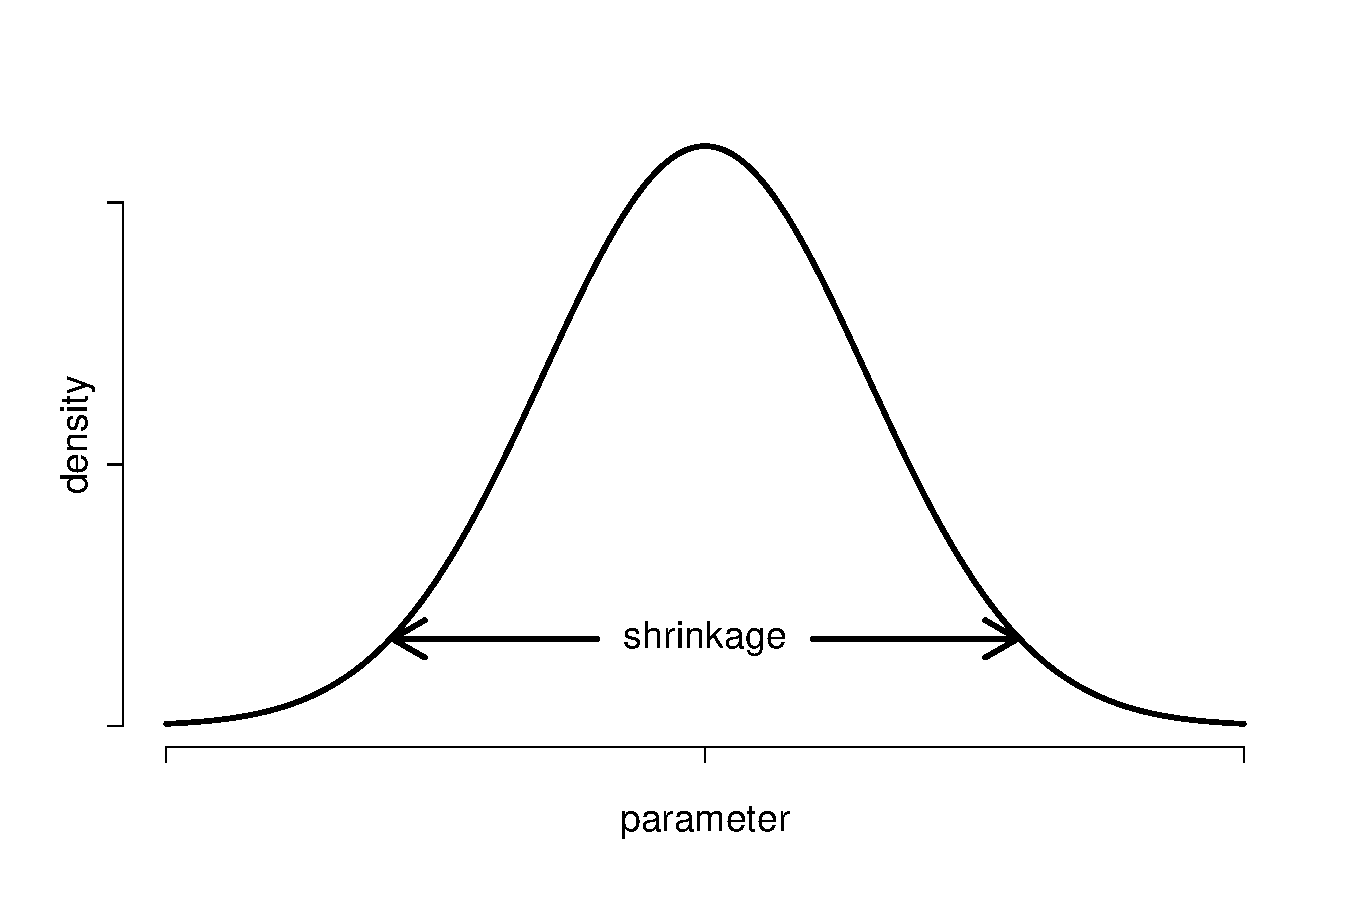
\includegraphics[scale=0.3]{shrinkage.pdf}
%\end{center}
%
%{\color{mcxs2}It introduces the trade off between the level of updating the prior knowledge by the data and exploiting predictive content of multiple variables.}
%
%\end{frame}



{\setbeamercolor{background canvas}{bg=purple}
\begin{frame}

\begin{adjustwidth}{-0.5cm}{0cm}
\vspace{8cm}\large
\textbf{{\color{mcxs1}Forecasting Australian real output growth and inflation} \\
{\color{mcxs5}using fat data}}
\end{adjustwidth}

\end{frame}
}




\begin{frame}{Forecasting Australian real output and inflation}

{\color{mcxs2}A dataset consisting of 117 quarterly macro-time series beginning in Q2 1985 was constructed by academics at Monash University and is available at} \href{http://www.ausmacrodata.org}{http://www.ausmacrodata.org}

\bigskip{\color{mcxs2}Two related publications describe the variables and use them for forecasting Australian real output and inflation.}

\bigskip\textbf{Information regarding dataset.}\scriptsize

{\color{mcxs2}Behlul, Panagiotelis, Athanasopoulos, Hyndman, Vahid (2017) The Australian Macro Database: An Online Resource for Macroeconomic Research in Australia}

\bigskip\textbf{Forecasting with 117 variables.}\scriptsize

{\color{mcxs2} Panagiotelis, Athanasopoulos, Hyndman, Jiang, Vahid (2019) Macroeconomic forecasting for Australia using a large number of predictors, International Journal of Forecasting}

\end{frame}



\begin{frame}{Forecasting Australian real output and inflation}

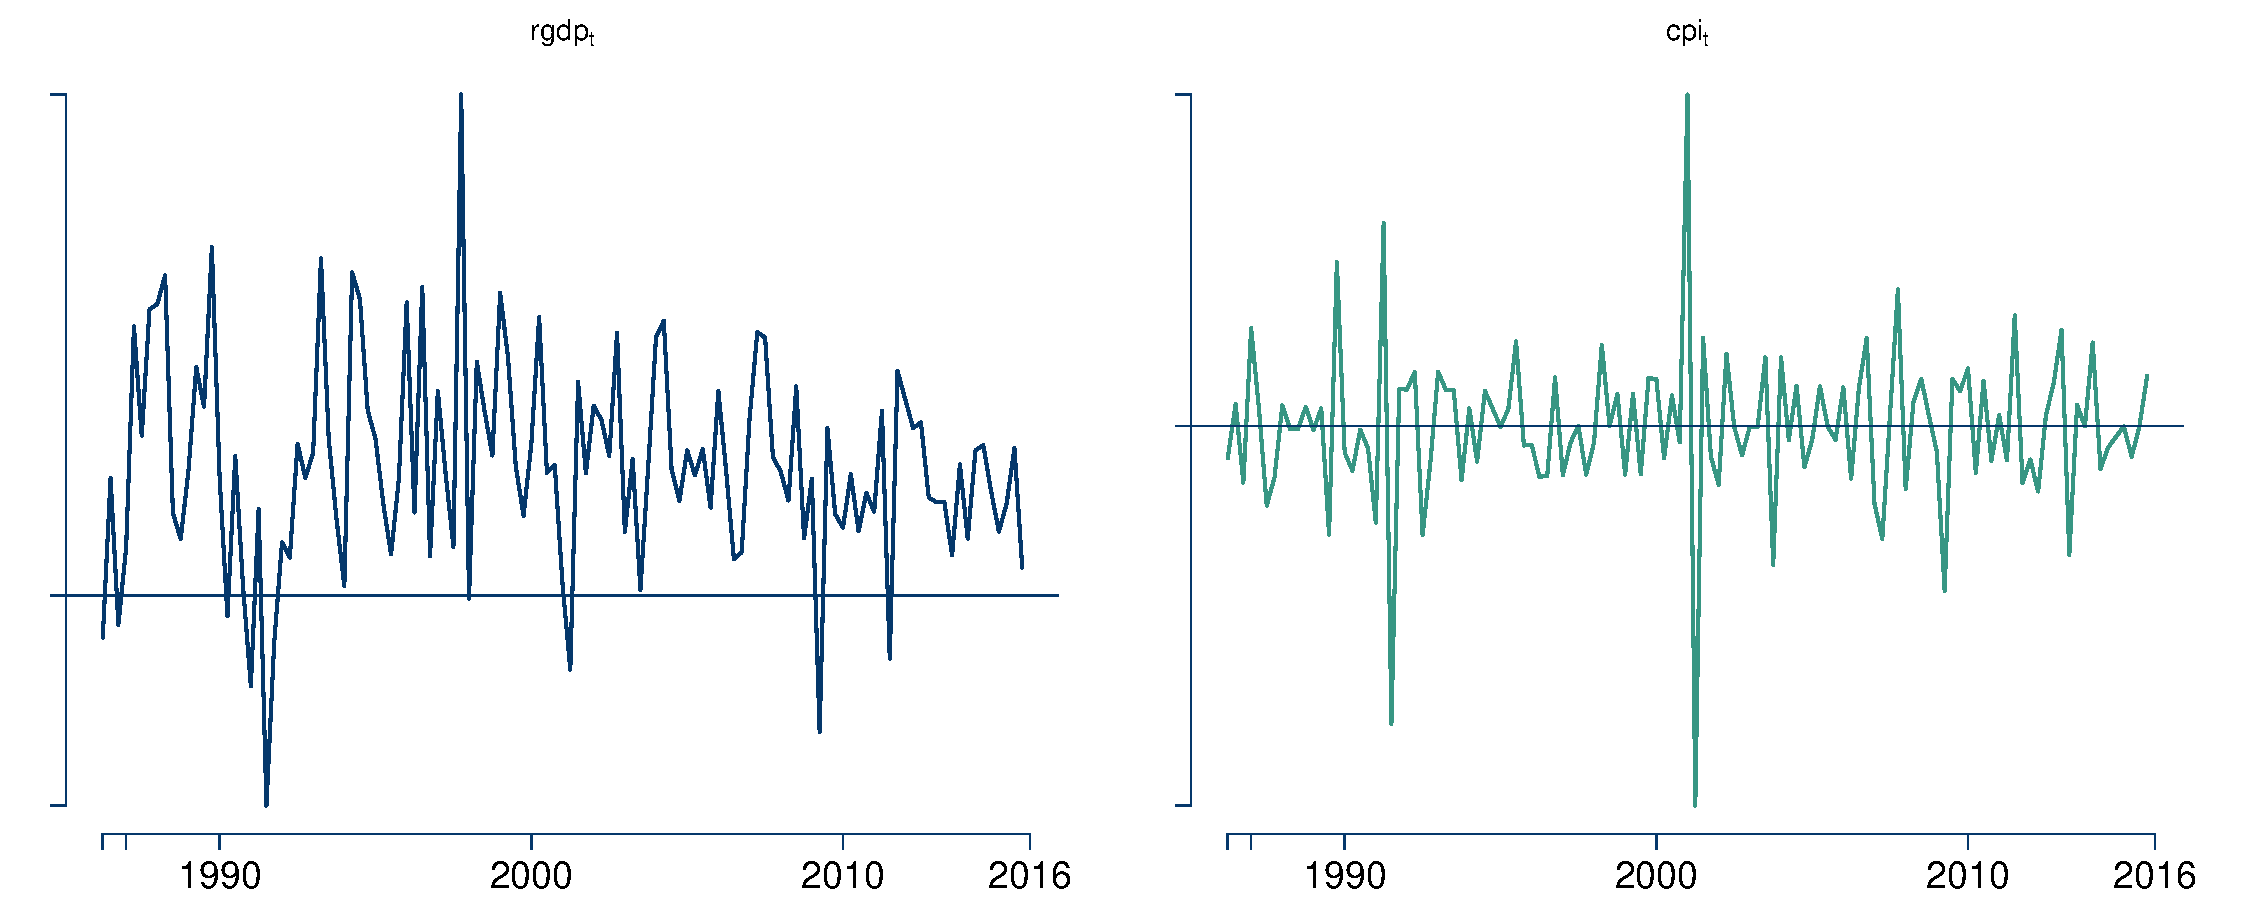
\includegraphics[scale=0.3]{data1.pdf}

$$rgdp_t = \Delta RGDP_t\qquad {\color{mcxs2}cpi_t = \Delta^2 CPI_t}$$

\bigskip\footnotesize{\color{mcxs2}A dataset consisting of 117 quarterly macro-time series beginning in Q2 1985 and finishing in Q1 2016 $T=120$ \href{http://www.ausmacrodata.org}{http://www.ausmacrodata.org}}

\end{frame}




\begin{frame}{Forecasting Australian real output and inflation}

{\color{mcxs2}The variables are transformed to stationary form by differentiation or log-differentiation.}

\bigskip\textbf{Minnesota prior mean.}

{\color{mcxs2}Therefore, the prior mean for matrix} $A$ {\color{mcxs2}is set to}
$$ \underline{A} = \mathbf{0}_{K\times N} $$
{\color{mcxs2}and implies a} {\color{purple}white noise} {\color{mcxs2}process} $ y_t = \epsilon_t $



\bigskip\textbf{Minnesota prior shrinkage.}

{\color{mcxs2}The overall shrinkage parameter} $\kappa_1$ {\color{mcxs2}is controlling the dispersion around a prior mean.}

\end{frame}









\begin{frame}{Forecasting Australian real output and inflation}

\textbf{Forecasting using two variables.}

\bigskip
\centering
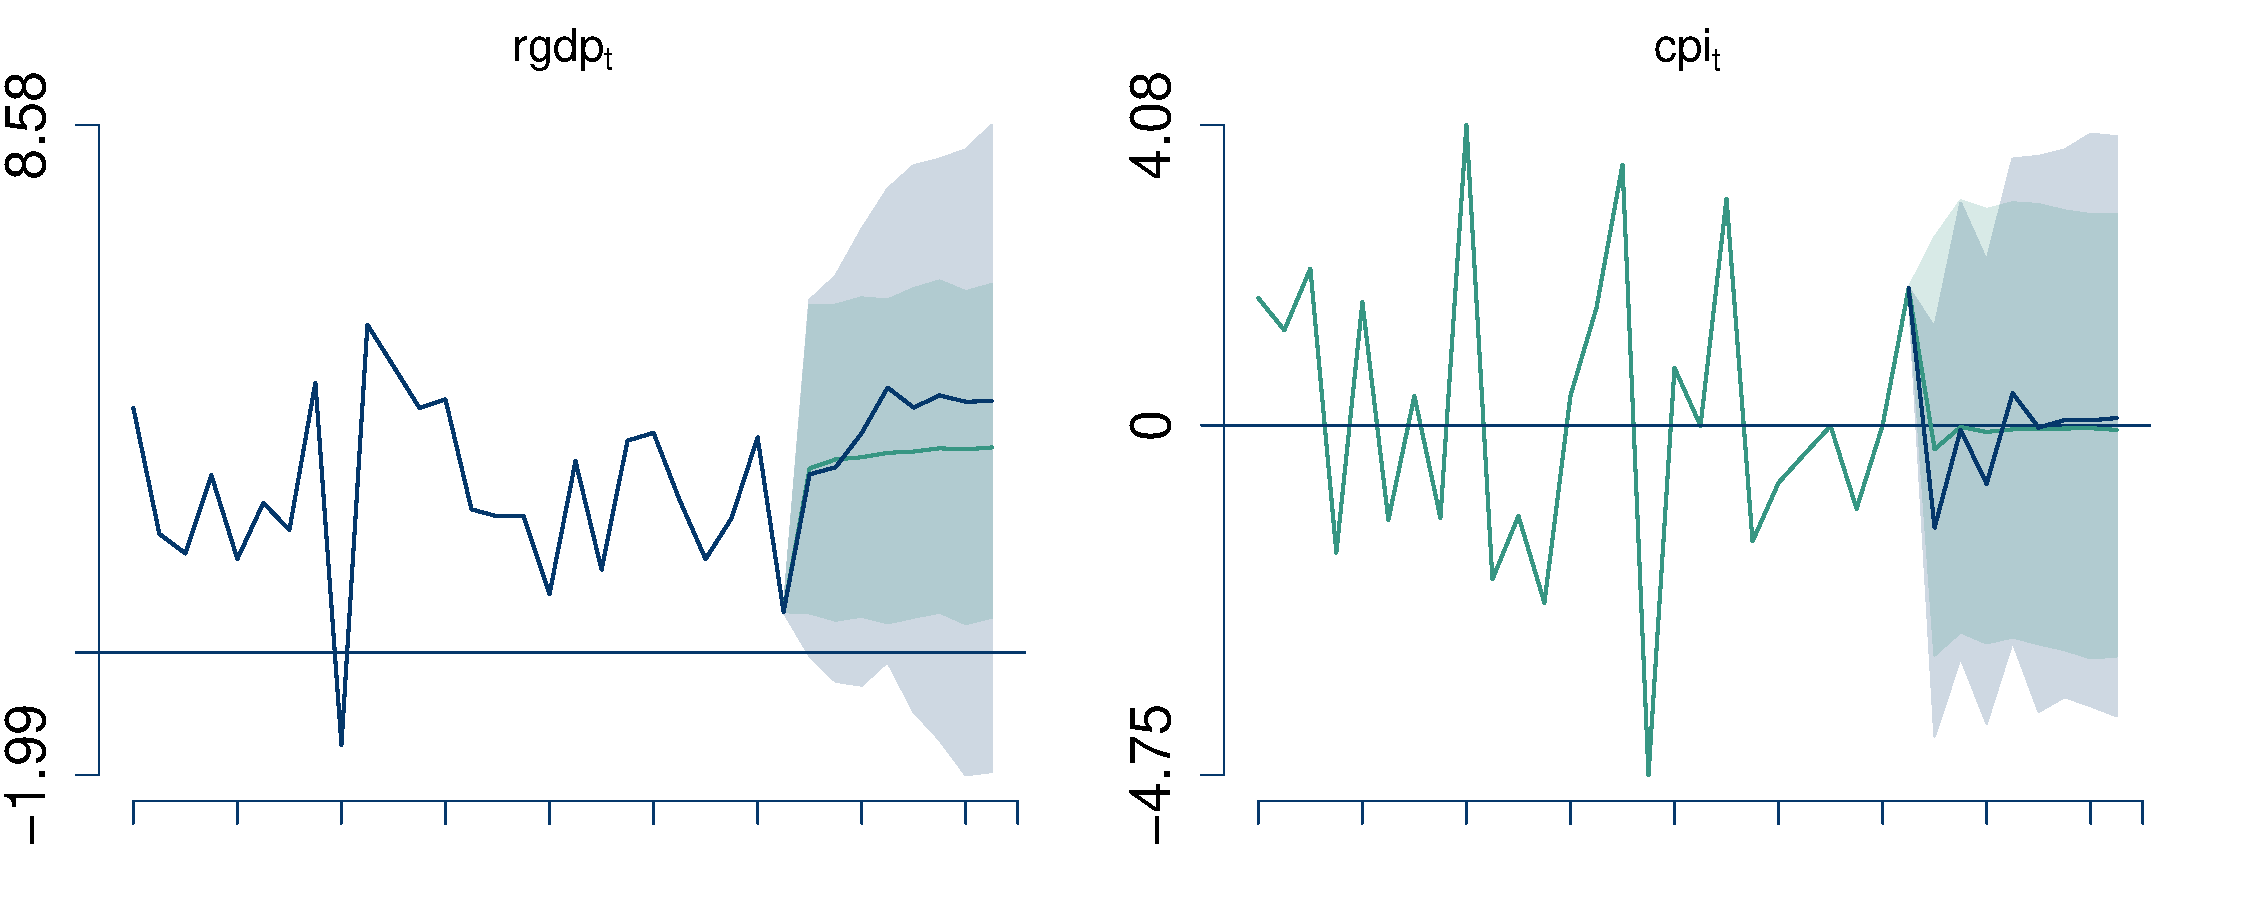
\includegraphics[scale=0.3]{forecasts-N2.pdf}

\bigskip{\color{mcxs1}Bayesian VAR(4) with Minnesota prior and $\kappa_1=1$}

{\color{mcxs2}Bayesian VAR(4) with Minnesota prior and $\kappa_1=0.02^2$}

\bigskip\footnotesize
2-year ahead mean forecasts and 68\% predictive intervals
\end{frame}




\begin{frame}{Forecasting Australian real output and inflation}

\textbf{Forecasting using 117 variables.}

\bigskip
\centering
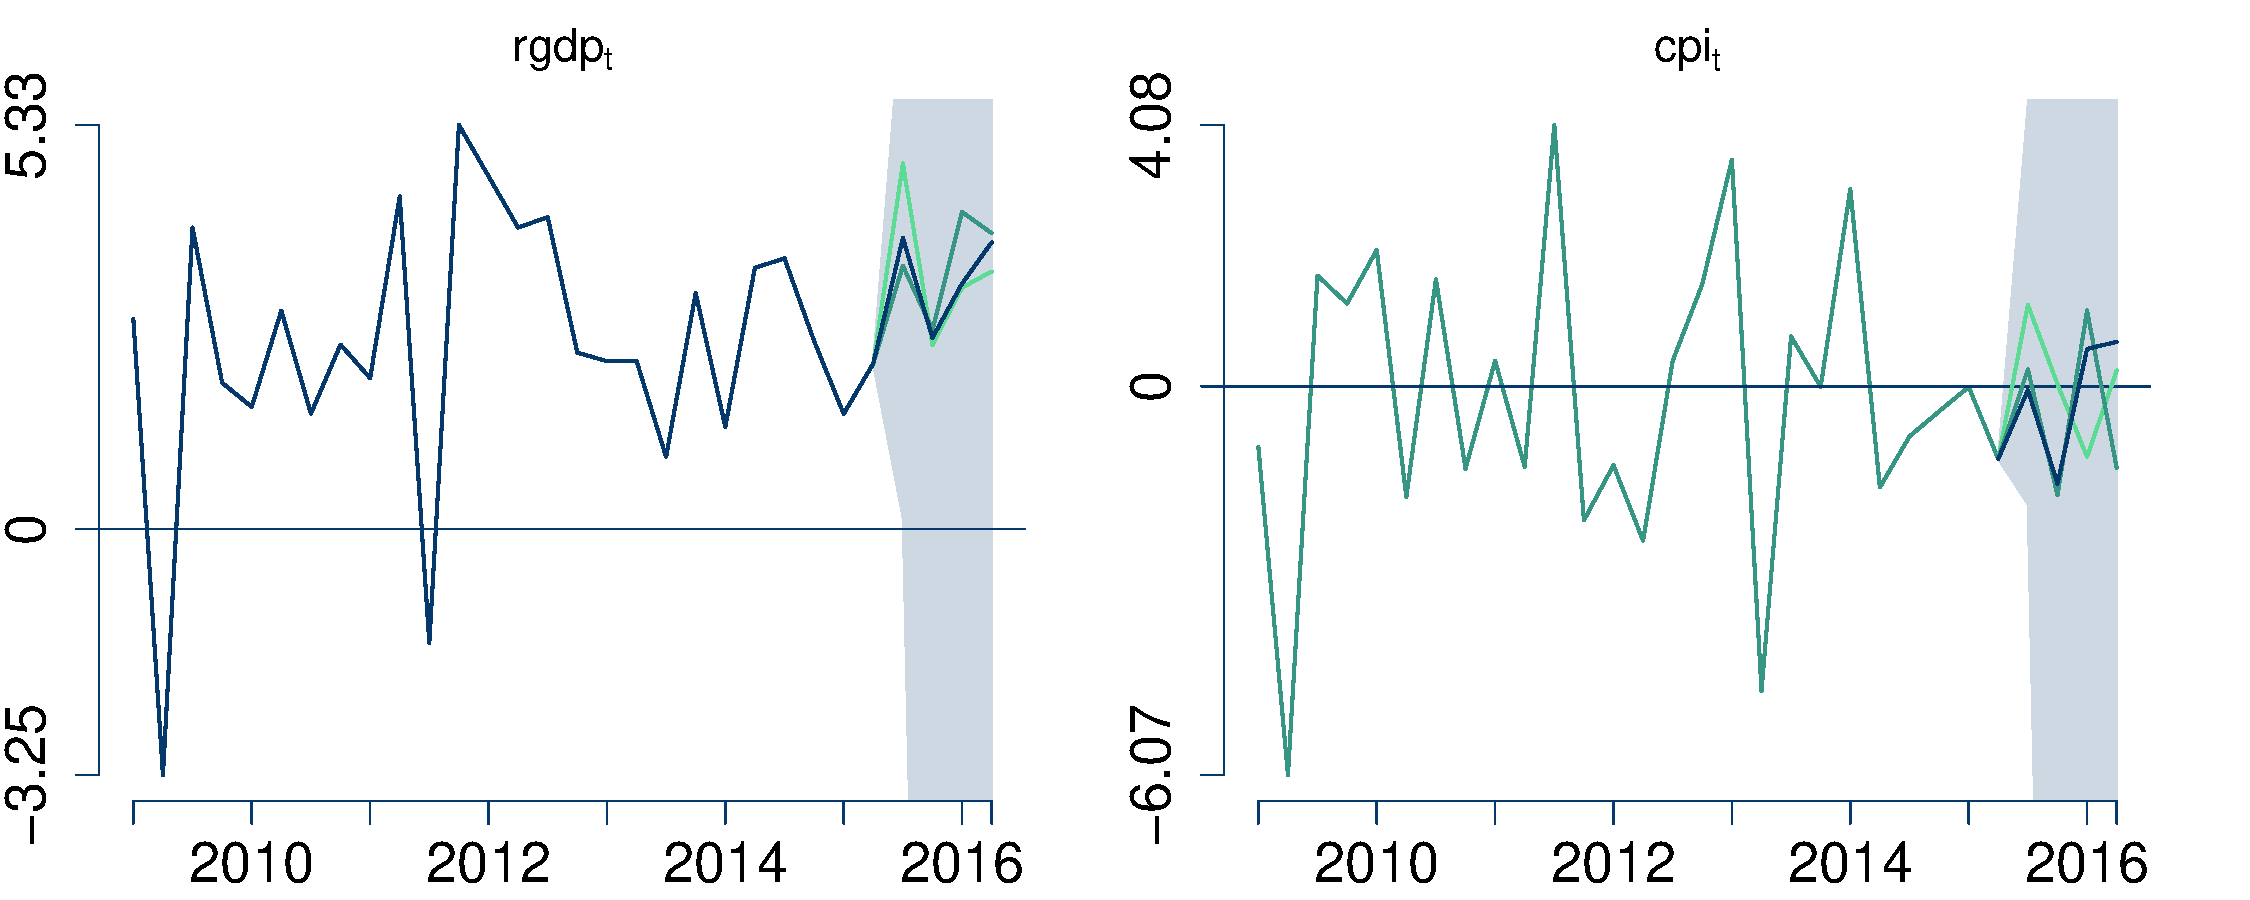
\includegraphics[scale=0.3]{forecasts-N117.pdf}

\bigskip{\color{mcxs3}Bayesian VAR(1) with Minnesota prior}

{\color{mcxs2}Bayesian VAR(2) with Minnesota prior}

{\color{mcxs1}Bayesian VAR(4) with Minnesota prior\\ \scriptsize
In this model, matrices $A$ and $\Sigma$ contain jointly 61,776 unique parameters.}

\bigskip\footnotesize
1-year ahead mean forecasts and 68\% predictive interval for VAR(1)

\end{frame}






{\setbeamercolor{background canvas}{bg=purple}
\begin{frame}{\color{mcxs1}Forecasting with large Bayesian VARs}
\begin{description}
\item[Bayesian VARs] {\color{mcxs5}are benchmark models for macroeconomic forecasting}

\bigskip\item[Dedicated prior specification] {\color{mcxs5}supports the identification and forecasting with fat data}

\bigskip\item[Feasible computations] {\color{mcxs5}thanks to application of shrinkage, Kronecker structure of covariances, and programming routines for big matrices}
\end{description}
\end{frame}
}

\end{document} 